%\documentclass[twocolumn,twoside]{article}
\documentclass[twoside,twocolumn, letterpaper]{article}
\usepackage{graphics}
\usepackage{color}
\usepackage{NatGenArtT}
%\usepackage{NatureLetT}
\usepackage{times}
\DeclareMathAlphabet{\msfsl}{OT1}{cmss}{m}{sl}
\DeclareMathAlphabet{\msfrg}{OT1}{cmss}{n}{sl}
\renewcommand{\baselinestretch}{1}
\addtolength{\oddsidemargin}{-.2cm}
\addtolength{\evensidemargin}{-1.2cm}
\addtolength{\textwidth}{1.5cm}
\addtolength{\topmargin}{-1.75cm}
\addtolength{\textheight}{3.5cm}
\renewcommand{\textfraction}{0.01}
\renewcommand{\topfraction}{0.99}
\renewcommand{\bottomfraction}{0.65}
\renewcommand{\floatpagefraction}{0.90}
\renewcommand{\dbltopfraction}{0.95}
\renewcommand{\dblfloatpagefraction}{0.80}
\renewcommand{\sfdefault}{phv}

%added commands YANG
\newcommand{\sme}[1]{\textcolor{red}{\bf #1}}
\newcommand{\yang}[1]{\textcolor{cyan}{\emph{\bf  #1}}}
\newcommand{\X}{\textcolor{red}{\bf X\,}}
\newcommand{\citex}{\textcolor{red}{\bf (CITE)\,}}
\newcommand{\jri}[1]{\textcolor{red}{ \emph{ #1}} }
\graphicspath{{Figure_Table/}} % Location of the graphics files

\makeatletter
\renewcommand{\footnotesep}{-2pt}
\makeatletter

\usepackage{fancyhdr}
\pagestyle{fancy}
\fancyhf{}

% fancy for Nature Genetics
\fancyhead[RO]{\begin{picture}(600,1)(10,20)\put(440,32) {\textcolor{Dgreen}{\large{\sfbf{ARTICLES}}}}\end{picture}}
\fancyhead[RE]{\begin{picture}(600,1)(10,20)\put(10,32)  {\textcolor{Dgreen}{\large{\sfbf{ARTICLES}}}}\end{picture}}
\fancyhead[C]{\begin{picture}(600,1)(10,20)\linethickness{50pt}\put(-43,52) {{\color{pTop}{\line(1,0){615}}}}\linethickness{0.5pt}\put(10,-678) {{\line(1,0){515}}}\end{picture}}

% fancy for Nature
%\fancyhead[RO]{\begin{picture}(600,1)(10,20)\put(460,46) {\textcolor{Dgreen}{\stbld{LETTERS}}} \put(10,46) {\textcolor{Dgreen}{\sf{NATURE}}} \end{picture}}
%\fancyhead[RE]{\begin{picture}(600,1)(10,20)\put(10,46) {\textcolor{Dgreen}{\stbld{LETTERS}}} \put(460,46) {\textcolor{Dgreen}{\sf{NATURE}}} \end{picture}}
%\fancyhead[C]{\begin{picture}(600,1)(10,20)\linethickness{25pt}\put(-43,54) {{\color{pTop}{\line(1,0){615}}}}\linethickness{0.5pt}\put(10,-678) {{\line(1,0){515}}}\end{picture}}

\fancyfoot[RO]{\thepage}
\fancyfoot[LE]{\thepage}

\renewcommand{\headrulewidth}{0pt}
\fancypagestyle{plain}{
    \fancyhf{}
}
\setcounter{footnote}{0}%

\title{Incorporation of Evolutionary Constraint Improves Genomic Prediction of Hybrid Phenotypes}


\author{
Jinliang Yang\thanks{Department of Plant Sciences, University of California, Davis, CA 95616, USA} $^,$\thanks{These authors contributed equally to this work} \hspace{0.5mm}, 
Sofiane Mezmouk$^{1,2,}$\thanks{Current address: KWS SAAT AG, Grimsehlstr. 31, 37555 Einbeck, Germany} \hspace{0.5mm}, 
Andy Baumgarten\thanks{DuPont Pioneer, Johnston, IA 50131, USA} \hspace{0.5mm}, 
Edward S. Buckler\thanks{US Department of Agriculture, Agricultural Research Service, Ithaca, NY 14853, USA} \hspace{0.5mm}, 
Katherine E. Guill\thanks{US Department of Agriculture, Agricultural Research Service, Columbia, MO 65211, USA} \hspace{0.5mm},
Michael D. McMullen$^{6,}$\thanks{Division of Plant Sciences, University of Missouri, Columbia, MO 65211, USA} \hspace{0.5mm},
Rita H. Mumm\thanks{Department of Crop Sciences, University of Illinois at Urbana-Champaign, Urbana, IL 61801, USA} \hspace{0.5mm},
and Jeffrey Ross-Ibarra$^{1,}$\thanks{Center for Population Biology and Genome Center, University of California, Davis, CA 95616, USA} $^,$\thanks{Correspondence should be addressed to J.R.-I. (rossibarra@ucdavis.edu).}\hspace{0.5mm}
}
\date{\small Manuscript intended for \emph{Nature Genetics}, \today}



\usepackage[sort&compress]{natbib}
\bibpunct{}{}{,}{s}{}{\textsuperscript{,}}

\usepackage{amsmath}
\usepackage{graphicx}

\begin{document} 
\maketitle

\begin{abstract}
\noindent \bf
\noindent
Complementation of deleterious alleles has long been proposed as a major contributor to the hybrid vigor observed in offspring of inbred parents. 
We test this hypothesis using evolutionary measures of sequence conservation to ask whether incorporating information about putatively deleterious alleles can inform genomic selection (GS) models and improve phenotypic prediction.
We measured a number of agronomic traits in both the inbred parents and hybrids of an elite maize partial diallel population. 
We resequenced the parents of the population, using genomic evolutionary rate profiling (GERP) to identify constrained sites across more than 86 Mb sites across the genome.  
We identifed haplotype blocks using an identity-by-decent (IBD) analysis and scored these blocks on the basis of segregating putatively deleterious variants. 
As a result, incorporating sequence conservation improves prediction accuracies in a five-fold cross-validation experiment for several traits \emph{per se} as well as heterosis for those traits. 
These results provide strong empirical support for the simple complementation model of heterosis, and demonstrates the utility of incorporatin functional annotation and its potential usage in phenotypic prediction and plant breeding. 

\end{abstract}

\vspace{6mm}




%%%%%%%%%%%%%%%%%%%%%%%%%%%%%%%%%%%%%%%%%%%%%%%%%%%%%%%%%%%
\noindent %\textbf{Why we care about deleterious variants. Discuss results of Mezmouk 2014. We are extending this in three ways}  
%\begin{itemize}
%  \item all deleterious SNPs not just coding
%  \item genome-wide not just reduced representation
%  \item using GS to test whether they improve prediction
%\end{itemize}

The phenomenon of heterosis or hybrid vigor has been observed across many species, from yeast \citep{Shapira2014} to plants \citep{shull1908composition} and vertebrates \citep{Gama2013}. 
Hybrid vigor is particularly important in agriculture, where hybrid breeding is fundamental to the production of a number of crops including both rice \citex and maize \citex .
A number of hypotheses have been put forth to explain the phenomenon, including gene dosage \citep{birchler2003search}, overdominance \citep{east1936heterosis, schwartz1973single, krieger2010flowering}, 
%pseudo-overdomiance \cite[]{graham1997characterization, McMullen2009}, 
and epistasis \citep{minvielle1987dominance, schnell1992multiplicative}. 
Complementation of recessive deleterious alleles, however, remains the simplest genetic explanation \citep{Charlesworth2009}, and one that is supported by considerable empirical evidence \citex \citep{xiao1995dominance, frascaroli2007classical}.
\jri{i'm not sure these are all appropriate. huang2015genomic for example i think doesn't actually measure heterosis, they just do GWAS on hybrids. and frascaroli if I read it right says that heterosis for grain yield is mostly overdominance (dominance $>1$).}

%One of the best studied examples of hybrid vigor is that of maize. 
%Hybrid maize has formed the basis of modern maize agriculture since the early 20th century \cite[]{crow1998}. 

%Cr the benefits of cross-fertilization or hybridization were not unknown, it was not until the early 20th century that East, Shull, and others demonstrated the utility of hybrid breeding for  in the past, it was not until the early 20th century that hybridwork of Shull, East, and others that it's significance for agriculture was well appreciated \citex.
%Now, hybrid seed makes up the vast majority \jri{in progress, still reading}


%Deleterious alleles were arisen from new mutations during meiosis. In maize, about 90 new mutations were generated per meiosis \cite[]{Clark2005}, majority of which were deleterious according to empirical estimates \cite[]{Joseph2004}. In a natural outcross population, the negative effects on fitness of these deleterious alleles make them subject to be selection against, which lead the deleterious alleles to be maintained in a low frequency \cite[]{Eyre-Walker2007}. But the deleterious alleles could not be completely purged. 

%In maize, the total number of mildly deleterious mutations is substantial because of the exponential growth of population size after domestication. The modern breeding probably aims to remove these deleterious mutations and pyramiding beneficial alleles for agronomical purposes. In practice, the relatively homogeneous maize germplasm pool was artificially divided into different heterotic groups \cite[]{Heerwaarden2012}. It enabled the improvement of germplasm pools to be conducted in a parallel fashion, and therefore, facilitated the breeding efficiency. Using this hybrid breeding approach, the maize yield has been steadily improved since the early 20th century \cite[]{duvick2001biotechnology}. However, removing deleterious mutations in low recombination regions or in tightly linked regions become less effective. Studies indicated that residual heterozygosity correlates negatively with recombination \cite[]{Gore2009, McMullen2009} and the low recombination is effective over long period of time \cite[]{Haddrill2007}. As a consequence, the deleterious alleles would be accumulated in the low recombination regions, such as the pericentromeric regions in maize, and the vigorous performance could be realized by combining two sets of non-deleterious or beneficial alleles in repulsion state, thus lead to pesudo-overdominance. A recent QTL study identified loci controlling for heterosis are enriched in centromeric regions \cite[]{Lariepe2012}, which partly support this pesudo-overdominance hypothesis.

%Despite the importance of deleterious alleles in contributing to heterosis, they have not been systematically investigated probably because of their low frequencies in the population and mostly exhibiting minor effects. Here, we employed a genomic selection (GS) approach to simultaneously estimate genome-wide deleterious variants in a half diallel population. The diallel population was composed of a set of hybrids, which enabled us to explore different modes of inheritance of the deleterious variants. And the study can be conducted with millions of variants but using relative little sequencing efforts. In our previous study, deleterious SNPs were found to be enriched in a SNP set identified by GWAS \cite[]{Mezmouk2014}. The deleterious variants in the study were defined as non-synonymous mutations in the coding regions. Clearly, deleterious variants are not limited to coding regions. Here, we expanded the characterization of deleterious variants to genome-wide using genomic evolutionary rate profiling (GERP) \cite[]{Cooper2005}. By incorporating GERP information in GS models, we demonstrated the prediction accuracies were significantly improved not only for some traits \emph{per se}, but aslo for some heterosis transformations (especially for traits exhibiting high levels of hereosis). Further studies indicated that joint effects of deleterious alleles with additive and dominant modes of inheritance may contribute to heterosis.



%%%%%%%%%%%%%%%%%%%%---phenotype------%%%%%%%%%%%%%%%%%%%%%% 
\begin{figure*}[tb]   
  \begin{center}
   \vspace{-2mm}
   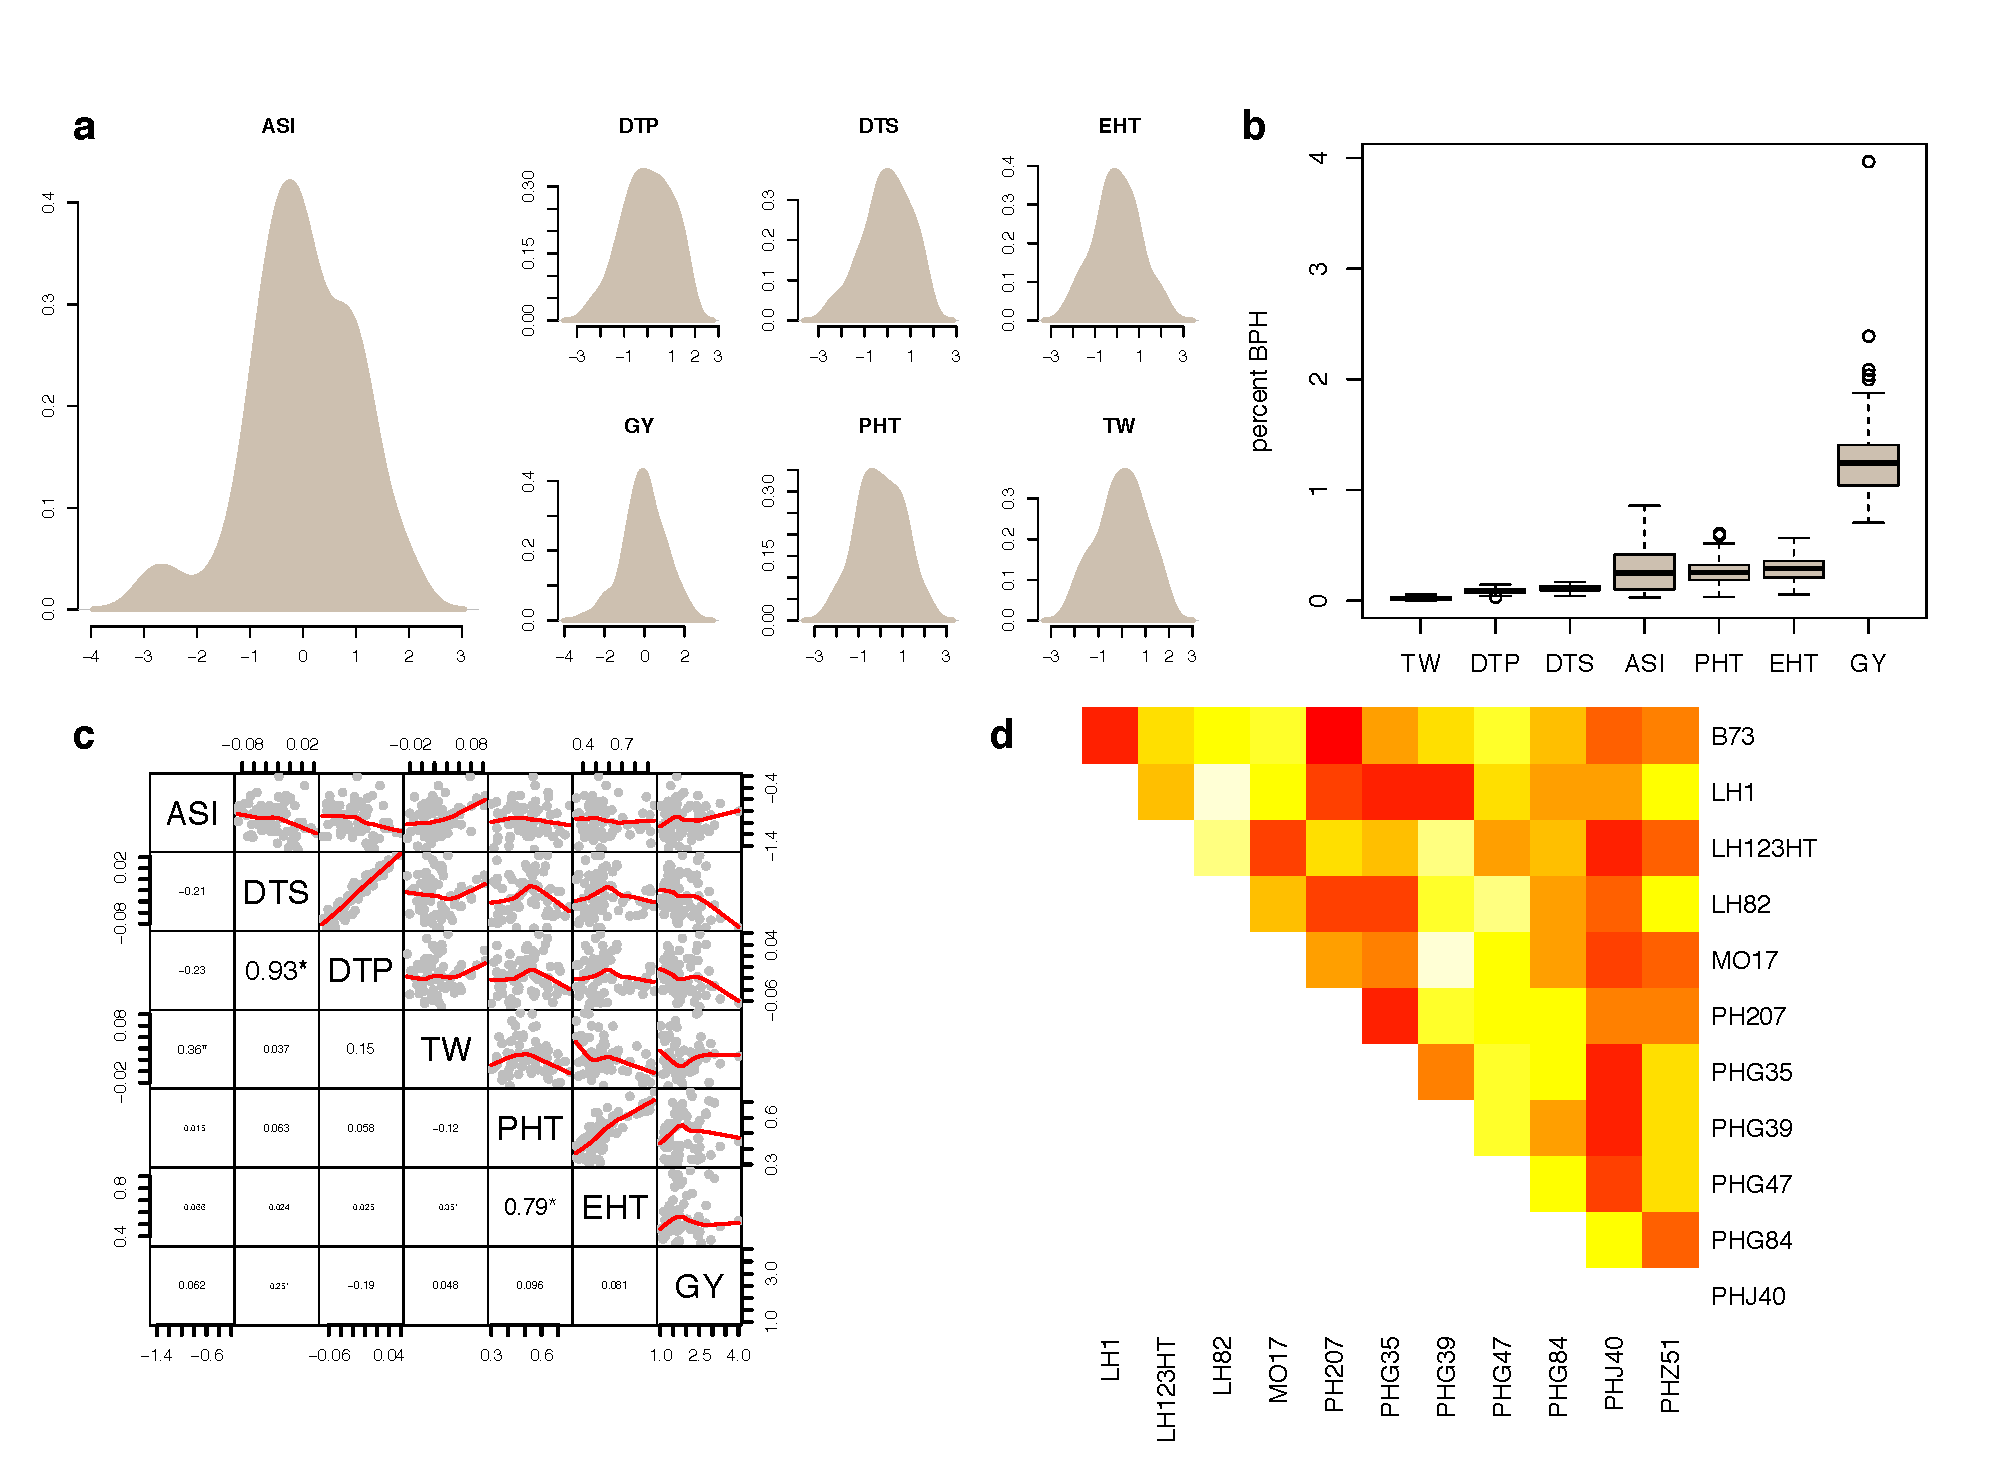
\includegraphics[width=0.8\linewidth]{Fig1_pheno.pdf}
   \renewcommand{\baselinestretch}{0.9}
   \vspace{-3mm}
   \caption{({\bfseries a-b}) Phenotypic variability in an elite maize partial diallel. (Left) Density plots of the BLUE values for the seven phenotypic traits. On the x-axis, the phenotypic values were normalized. \jri{does this include hybrids or just parents?} (Right) Boxplot of percent best parent heterosis (pBPH). In the plot, ASI was calculated using pBPHmin and the other six traits were calculated using pBPHmax. \jri{i sort of messed up the formatting of this figure. maybe include as two separate figures? do as a panel? the boxplot should be in the main text though. }} 
\vspace{-4mm}
    \label{fig:pheno}
  \end{center}
\end{figure*}
%%%%%%%%%%%%%%%%%%%%%%%%%%%%%%%%%%%%%%%%%% FIGURE


%%%%%%%%%%%%%%%%%%%%%%%%%%%%%%%%%%%%%%%%%% RESULTS %%%%%%%%%%%%%%%%%%%%%%%%%%%%%%
\section*{RESULTS}
\subsection*{Genetic values, heritability and heterosis}

A partial diallel population was created using 12 maize inbred lines. Two of them are important public inbreds, B73 and Mo17, the former of which was selected as the maize reference genome \citep{schnable2009b73}. And the other ten are proprietary inbreds (LH1, LH123HT, LH82, PH207, 4676A, PHG39, PHG47, PHG84, PHJ40, and PHZ51) that have expired from Plant Variety Protection Act (PVPA) \citep{nelson2008molecular} and represent much of the lineage of key heterotic germplasm pools used in present-day commercial corn hybrids.
From this population, phenotypic data were collected for seven traits of interest during 2009-2011: anthesis-silking interval (ASI, in days), days to 50\% pollen shed (DTP), days to 50\% silking (DTS), ear height (EHT, in cm), grain yield adjusted to 15.5\% moisture (GY, in bu/A), plant height (PHT, in cm), and test weight (TW, in pounds).

Best linear unbiased estimators (BLUEs) for genotypes of the seven traits were derived from mixed linear models (\textbf{Supplementary Table 1}).
In the models, all fixed effects were significant (Wald test \emph{P} value $<0.05$) for all traits except ASI, for which the effect of replicates within environments were not significant. 
As shown in Figure \ref{fig:pheno}, BLUE values were normally distributed (Shapiro-Wilk normality test \emph{P} values $>0.05$). 
Broad sense heritability ($H^2$) for these traits ranged from 0.65 for ASI to 0.95 for PHT. \jri{can we add these as a supp. table for all traits, or list them all here?} $H^2$ for DTP, DTS, EHT, GY and TW are x, x, x, x and x, respectively.
Using the parental phenotypic data, we then estimated best-parent heterosis (BPH) for each trait.  
Because the selected inbred lines are commercially relevant and fairly elite in performance, hybrids in this population exhibit relatively low hybrid vigor (overall mean percent BPH = 0.3\% $\pm$ 0.4\%) for most traits except GY (mean percent BPH = 95\% $\pm$ 16\%, Figure \ref{fig:pheno}). 
Finally, general and specific combining ability (GCA and SCA) were estimated following \citep{Falconer1996}. 
GCA and SCA varied among traits (Table \ref{table:table_s2}), but B73, PHG47 and PHG39 showed the greatest GCA for grain yield. 


%\begin{figure}[htbp]
%\centering
%\includegraphics[width=\linewidth]{SFig_pBPH.pdf}
%\caption{Boxplot of percent best parent heterosis (pBPH). In the plot, ASI was calculated using pBPHmin and the other six traits were calculated using pBPHmax.}
%\label{fig:pBPH}
%\end{figure}


%%%%%%%%%%%%%%%%%%%%---phenotype------%%%%%%%%%%%%%%%%%%%%%% 
\begin{figure*}[tbh]   
  \begin{center}
   \vspace{-2mm}
   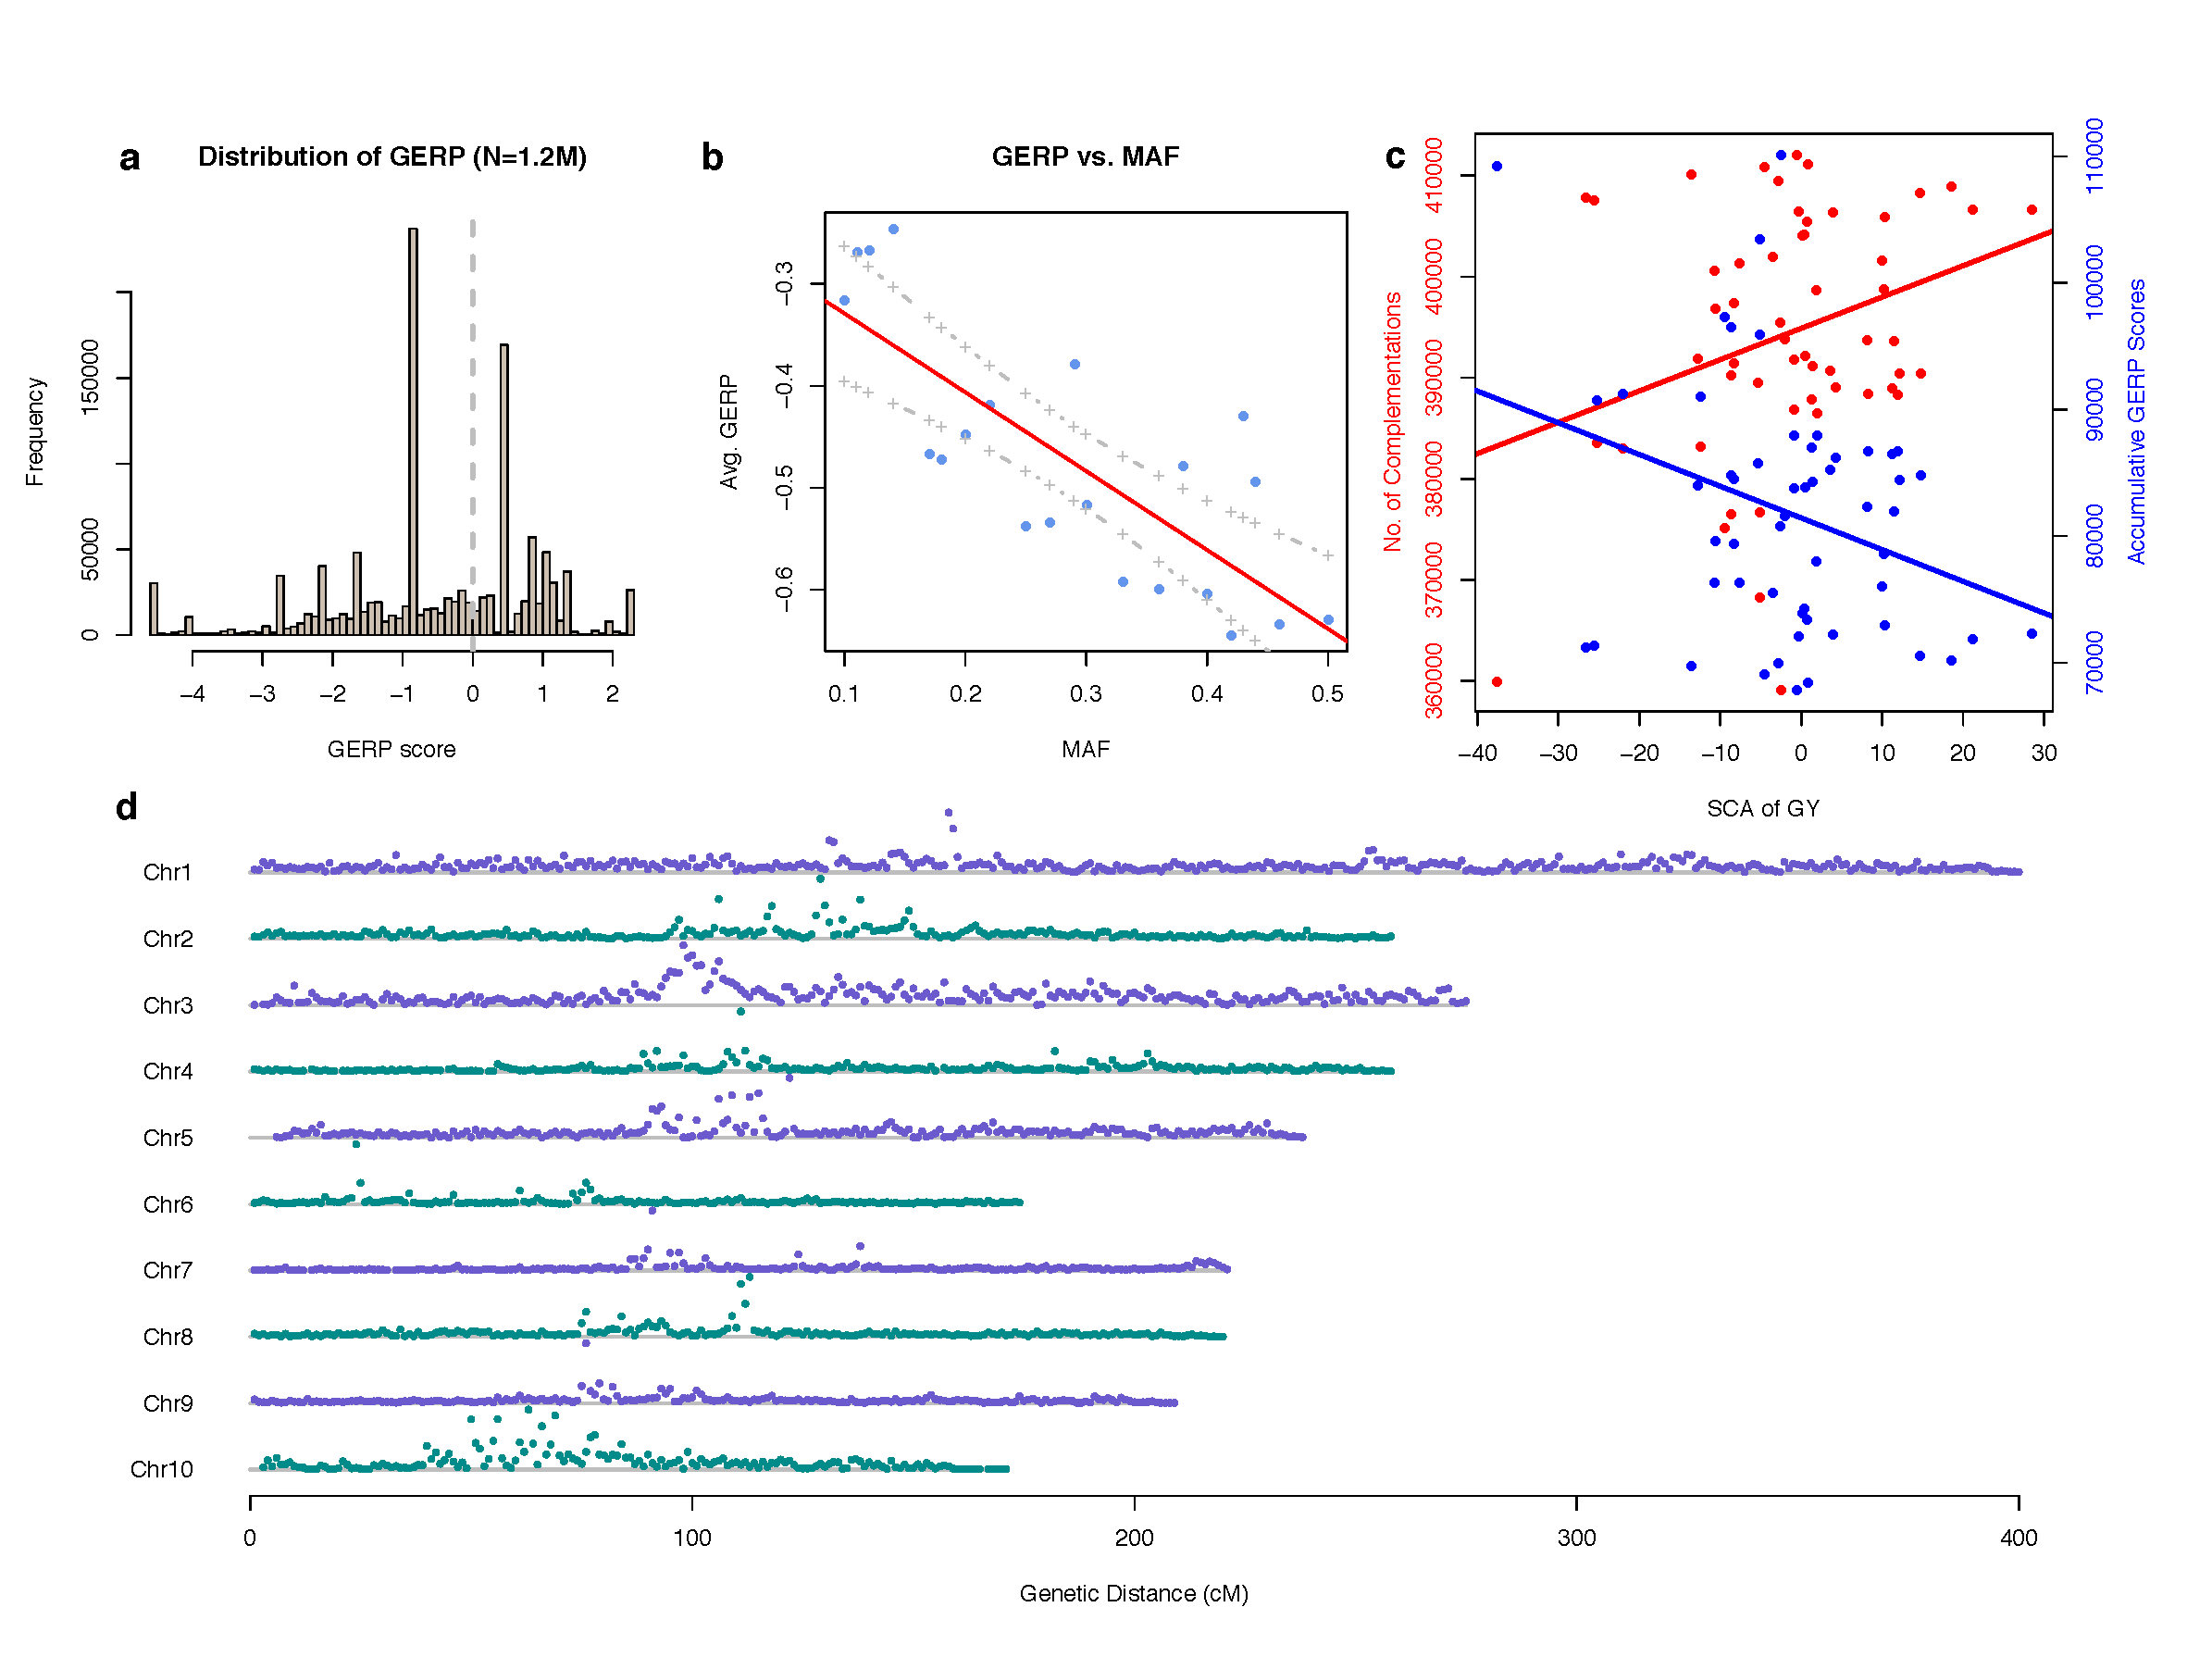
\includegraphics[width=0.8\linewidth]{Fig2_gerp.pdf}
   \renewcommand{\baselinestretch}{0.9}
   \vspace{-3mm}
   \caption{({\bfseries a-b}) Distribution of GERP scores and relationship between GERP scores and MAFs. \textbf{(A)} Histogram of GERP scores at $\sim$1.3 million SNPs. \textbf{(B)} Plot of average GERP scores in bins (bin size = 0.01) of minor allele frequency (MAF). Red and grey lines define the regression and its 95\% confidence interval.} 
\vspace{-4mm}
    \label{fig:gerp}
  \end{center}
\end{figure*}
%%%%%%%%%%%%%%%%%%%%%%%%%%%%%%%%%%%%%%%%%% FIGURE

\subsection*{Sequence variation and evolutionary constraint}

All twelve inbreds were sequenced to an average depth of $\sim$10X, resulting in a filtered set of 13.8 million SNPs. 
We estimated the allelic error rate using three independent data sets: for all individuals using 41,292 overlapping SNPs on the maize SNP50 bead chip \citep{Heerwaarden2012}; for all individuals using 180,313 overlapping SNPs identified through genotyping by sequencing (GBS) \citep{Romay2013}; and for B73 and Mo17 using the 10,426,715 SNP from the HapMap2 project \citep{Chia2012}.  Compared to corresponding SNPs identified by previous studies, a concordance rate of 99.1\% was observed. \jri{Sofiane: can we separate those numbers out by study? or just report for one study and mention that similar rates were seen in other studies? either way it would be nice to know what rate went with what data. also is concordance mean identical genotype? do we have minor allele rate (which is a bit more informative)? if not, skip it.} 

The minor allele frequency of SNPs at conserved sites was negatively correlated with GERP score (\textbf{Figure \ref{fig:gerp}a}; \emph{P} value $<$ 0.05, \emph{r} = $-0.8$), consistent with the idea that variants at sites with more positive GERP scores are more deleterious and more strongly impacted by purifying selection.

More than 86 million bp of the maize reference genome were annotated as conserved\citep{rodgers2015recombination}, with GERP scores $>0$. Nonetheless, 506,898 (or 0.6\%) of these sites were found to segregate among the 12 inbred parents of our diallel (\textbf{Figure \ref{fig:gerp}A} and \textbf{Supplementary Figure 1}).
On average, each inbred parent carried 179,144 putative deleterious variants, ranged from 156,386 (PHG35) to 195,959 (PHG84). Mo17 carried 189,241 putative deleterious variants, ranked as the third place. 

We calculated the number of complementation of these putative deleterious variants among F1 hybrids, except ones that have B73 as one of their parents. The best combination (Mo17 and PHG35) complemented each other at 412,042 sites, however, it still carried 94,856 homozygous putative deleterious alleles. The correlation of the complmentation significantly (Pearson correlation test, P-value = 0.02) correlated with the SCA of the GY trait and negative correlated with the cumulative deleterious scores (\textbf{Figure 2a}), which indicate hybrid combining ability might be determined by the complementation of deleterious alleles. \yang{correlation of the number of deleterious complementation and SCA, MPH and trait per se? Or just because of the genetic distance?}    

\yang{mean and variation of the deleterious variants per cM}
We also calculated mean deleterious variants per cM. As shown in (\textbf{Figure 2d}), large amount of deleterious variants were accumulated around the centromeric regions. 

\jri{this should be mentioned here but also in the results. is there any big variation?  some lines more than others? is mo17 worse than the pvps? given the comment below i added about linkage, can we calculate mean deleterious variants per cM?  that would be sweet to know and to point out that there are tons around the centromere. i think a bit more detail on distribution worthwhile since even Eli's paper is only using GBS. then add here a few sentences comparing to Eli's result and McMullen 2009.}

%%%%%%%%%%%%%%%%%%%%---phenotype------%%%%%%%%%%%%%%%%%%%%%% 
\begin{figure*}[tbh]   
  \begin{center}
   \vspace{-2mm}
   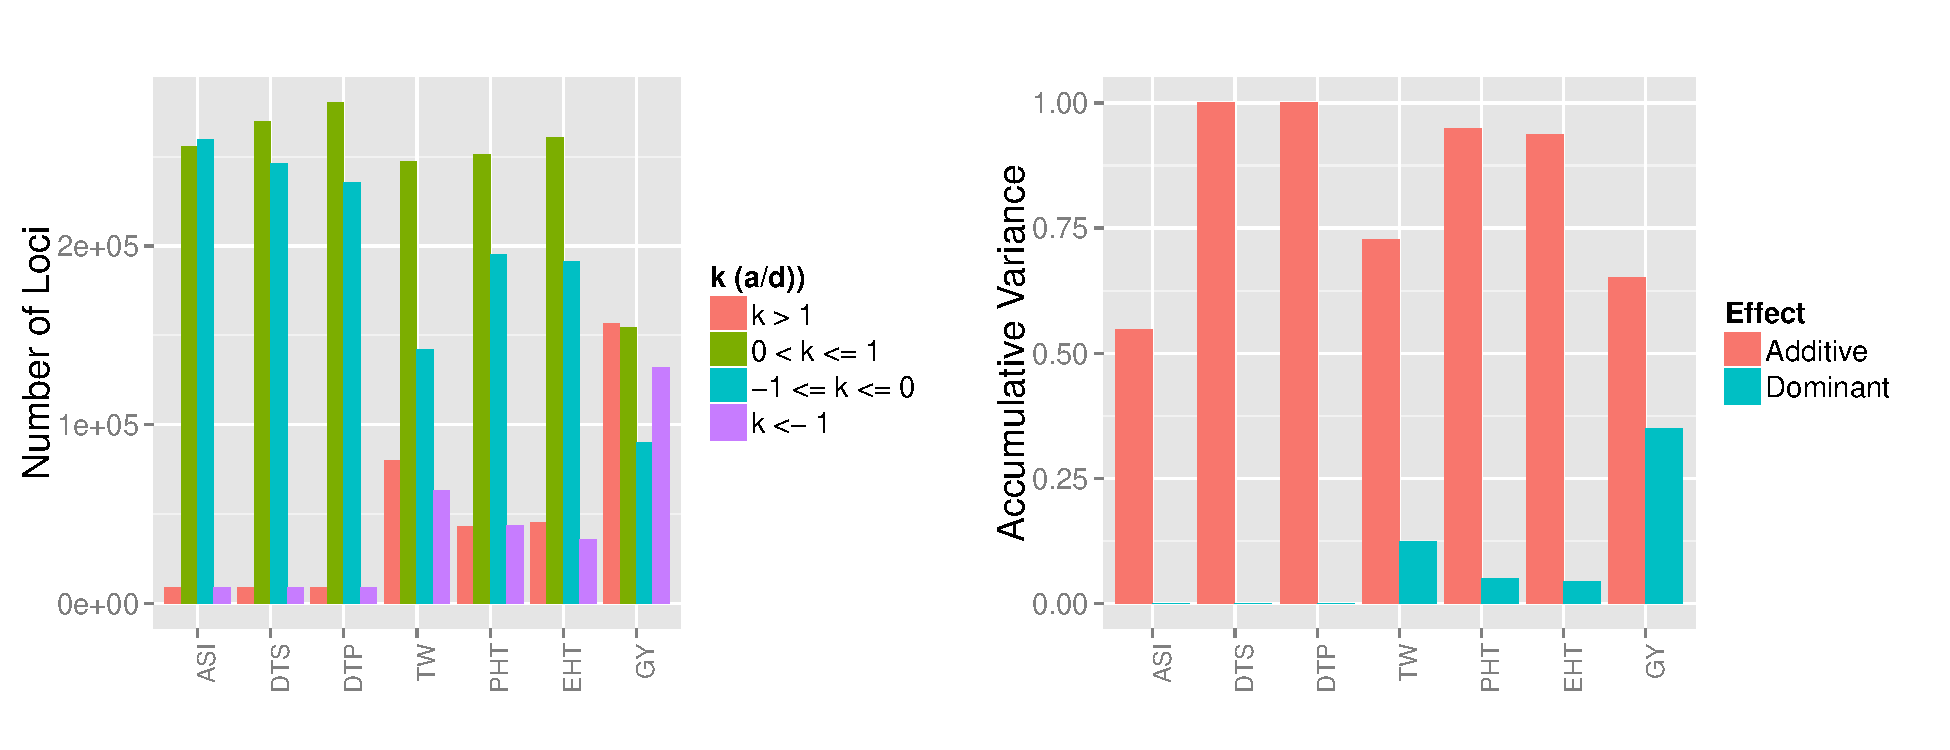
\includegraphics[width=0.8\linewidth]{Fig3_eff_var.pdf}
   \renewcommand{\baselinestretch}{0.9}
   \vspace{-3mm}
   \caption{({\bfseries a-b}) Distribution of GERP scores and relationship between GERP scores and MAFs. } 
\vspace{-4mm}
    \label{fig:effvar}
  \end{center}
\end{figure*}
%%%%%%%%%%%%%%%%%%%%%%%%%%%%%%%%%%%%%%%%%% FIGURE

\subsection*{Partition of the phenotypic variance}

A mixed linear model approach that partitions genetic values into additive (or allele subsitition effects) and dominant deviations were employed (\X Guo Hu et al.) to estimate the effects of GERP SNPs. According to Linch (\X), a degree of dominance (k) was defined as estimated dominant effect divided by estimated additive effect for a given GERP SNP. The value of $k > 1$ indicates the GERP SNP shows an overdominant effect; $0 < k < 1$ indicates a partial dominant effect; $-1 < k < 0$ indicates a partial recessive effect; and $k < -1$ indicates a underdominant effect. Note reference alleles at GERP sites were considered as beneficial alleles and the alternative alleles were deemed as deleterious alleles. Importantly, phenotypic traits with high level of heterosis have an excess of alleles showing dominant and overdominant effects. A correlation test showed that the number of constrast between dominance and overdominance loci and recessive and underdominance loci were singificated correlated with their levels of heterosis (\emph{P} value $<$ 0.01, \textbf{Figure 3a} ). Consistent with this, the accumulative variance explained by dominant effects were positively correlated with the levels of heterosis (\texttt{P} value $<$ 0.01,  \textbf{Figure 3b} )

Note the reasons that a large number of recessive loci were detected at GERP sites were: 1) the GERP may no the causal SNPs, the effects they accounted for might be the variants in LD with them; and 2) we did not apply any cutoff on effect detection, by chance a small negative dominant effects will be assigned;     





\subsection*{Phenotypic prediction}

 
The small sample size of our diallel and the general low frequency of deleterious SNPs precludes association-based approaches to evaluate the impact of variants on phenotypic variation.
To alleviate this limitation, we conceived a haplotype-based genomic selection approach in which we use estimates of evolutionary constraint across the genome to sum the individual effects of deleterious alleles within IBD blocks.

under additive, dominant and incomplete dominant models (see \textbf{Methods and Supplementary Figure 2}). %\ref{fig:gerpibd}). 

A Bayesian-based statistical method (BayesC) \citep{habier2011extension} using a 5-fold cross-validation approach was was employed for model training. 
In general, average prediction accuracies were higher using the additive model (mean \emph{r} = 0.81 and 0.49 for traits \emph{per se} and BPH) than the dominant model (mean \emph{r} = 0.70 and 0.42), and accuracies for heterosis traits were lower than for traits \emph{per se} (Table \ref{table:table_s3}).  A student-t test was employed to compare the mean prediction accuracies between data with real GERP information and data with permutated GERP. To account for multiple traits and multiple transformations, the FDR approach was used to correct the obtained P-values. As a result, incorporating evolutionary constraint information improved prediction accuracy for ASI and PHT \emph{per se} under an additive model and for ASI under a dominant model (FDR $<$ 0.05, Figure \ref{fig:gerpall} A and B).
GERP scores also improved prediction accuracies of heterosis (BPH) for GY under the additive model and DTP, DTS and TW under the dominant model (FDR < 0.05, Figure \iffalse\ref{fig:gerpall}\fi C and D). 
To rule out the possible confounding of high GERP scores and genic annotations, we re-permuted the data using only deleterious (GERP $> 0$) genic SNPs.  
Though this resulted in fewer SNPs (316, 983), the model prediction accuracies remained significantly improved for GY \emph{per se} under the additive model and for BPH of GY and PHT under the additive model (Figure \iffalse\ref{fig:genicsnp}\fi and \emph{Supplementary Table}). %\ref{table:table_s4}).   

%It was argued that SNPs in genic regions might have higher GERP scores than those in non-genic regions. The circular shuffling permutations may shift the high GERP scores to non-genic regions. If that is the case, the approach tended to weigh more on genic SNPs. To rule out this possibility, we elected SNPs with GERP scores >0 in genic regions only and did the circular shuffling to assign GERP scores to the same set of the selected SNPs. By doing this, the method will not take advantage of genomic positional information any more. Noted that in this study less number of SNPs was selected (N = 316, 983). Nevertheless, model prediction accuracies were significantly improved for traits \emph{per se} of GY under the additive model. For heterosis transformations, prediction accuracies were significantly improved for BPH of GY and PHT under the additive model and the prediction accuracy was significantly improved for pBPH of GY (Figure \ref{fig:genicsnp} and Table S4).   


%%%%%%%% ----- BEAN PLOT using all GERP SNPs-------- %%%%%%%%%%%
\begin{figure}[htbp]
\centering
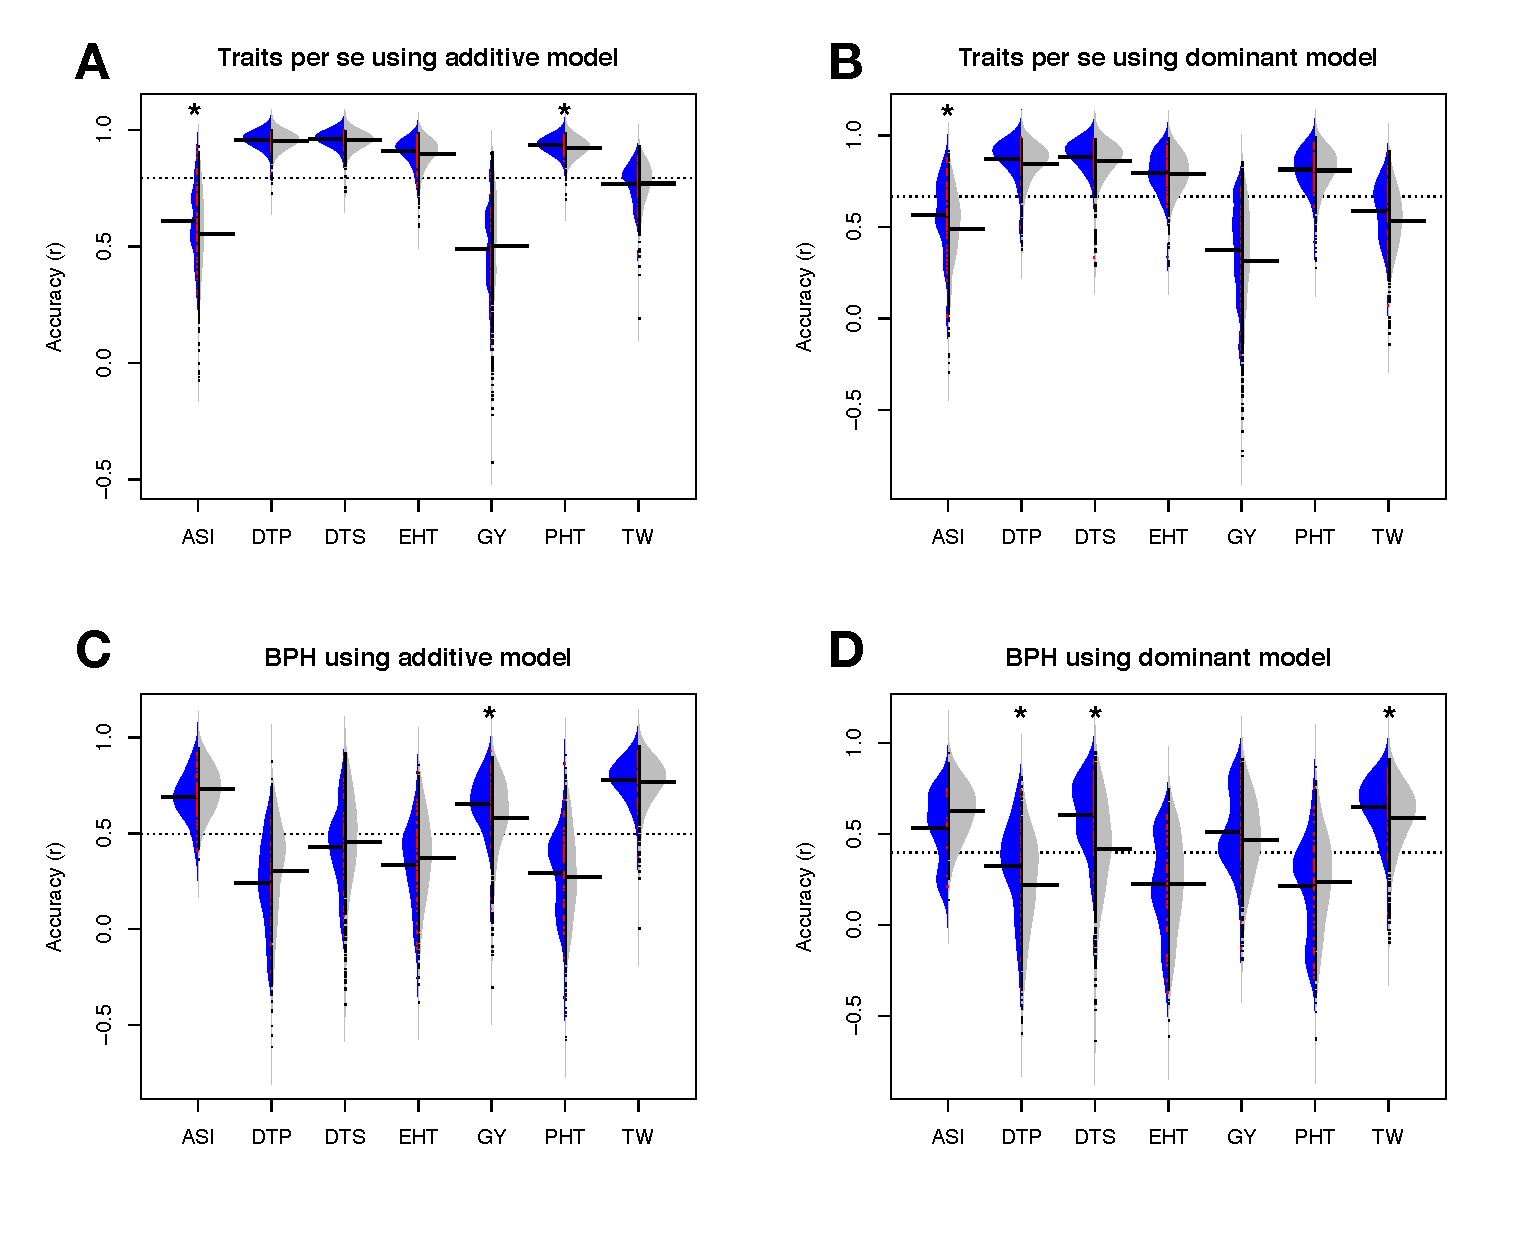
\includegraphics[width=\linewidth]{Figure_gerpall_m.pdf}
\caption{Beanplots of cross-validation accuracies using SNPs with positive GERP scores. Cross-validation experiments were conducted using selected SNPs and permuted data for traits \emph{per se} (\textbf{A, B}) and BPH (\textbf{C, D}) under additive (\textbf{A and C}) and dominant (\textbf{B and D}) models. Accuraries from the real data were plotted on the left (blue) and permutation results on the right (grey). Horizotal bars indicate mean accuracies for each trait and the grey dashed lines indicate the overall mean accuracy. Stars indicate significantly (FDR < 0.05) higher cross-validation accuracies.  \jri{need to explain red and black points}}
\label{fig:gerpall}
\end{figure}
%%%%%%%% ------------- %%%%%%%%%%%



\subsection*{Posterior phenotypic variance explained and model comparisons}

To learn why the prediction performace varied among traits \emph{per se} and heterosis, we obtained the posterior variance explained by our models using the complete set of data. 
As shown in Figure \ref{fig:h2}, additive models explained more phenotypic variance for traits \emph{per se} of DTP, DTS, EHT and PHT; but explained less phenotypic variance for heterosis (BPH) of ASI, GY and TW. 
In contrast, a larger proportion of the phenotypic variance could be explained by the dominant models for heterosis (BPH) of ASI, GY and TW. \jri{is this correct? the figure looks to me to disagree with this statement.}
This difference was particularly striking for grain yield under the dominant model, where only 3\% of the variance in trait \emph{per se} could be explained but 61\% of the variance in BPH was explained. \jri{I think a sentence or two here connecting variance explained with prediction accuracy would be helpful}

Heterosis transformations are largely determined by the accuracies of the parental phenotypes. 
To control for uncertainty of parental phenotypes, we estimated combining ability \jri{do we need to explain what this is and the difference between SCA and GCA?} directly from the hybrid population itself.
We extracted the breeding values estimated under both additive and dominant models using our haplotype blocks and incorporating GERP scores. 
We then applied the following models:
\begin{equation}
Y_{ij} = \mu + GCA_{i} + GCA_{j} + \varepsilon
\label{eq:refname1}
\end{equation}
\begin{equation}
Y_{ij} = \mu + GCA_{i} + GCA_{j} +  G_{ij} + \varepsilon
\label{eq:refname2}
\end{equation}
\begin{equation}
Y_{ij} = \mu + GCA_{i} + GCA_{j} + SCA_{ij} + \varepsilon
\label{eq:refname3}
\end{equation}
\begin{equation}
Y_{ij} = \mu + GCA_{i} + GCA_{j} + SCA_{ij} + G_{ij} + \varepsilon
\label{eq:refname4}
\end{equation}
where 
$Y_{ij}$ is the BLUE value of the hybrid crossed between the $i^{th}$ inbred and $j^{th}$ inbred; 
$\mu$, the overall mean; 
$GCA_{i}$, the general combining ability of the $i^{th}$ inbred;
$GCA_{j}$, the general combining ability of the $j^{th}$ inbred;
$SCA_{ij}$, the specific combining ability of between the $i^{th}$ and $j^{th}$ inbreds;
$G_{ij}$, breeding values estimated by our GS model for hybrid crossed between the $i^{th}$ inbred and $j^{th}$ inbred; 
$\varepsilon$, the model residuals.

Consistent with the previous analysis, haplotype blocks coded with the dominant mode of inheritance significantly improved the fit of models for heterosis for ASI and GY (equation \ref{eq:refname1} vs. equation \ref{eq:refname2}, ANOVA \emph{P} value $<0.05$, Table \ref{table:table_s5}). \jri{i'm having trouble following here.  GY gives a p of 0.04 which is not significant after bonferonni (maybe after FDR?) under the dominant model, but DOES give a significant p<4E-16 under the additive model. why not mention/discuss that? }
Comparison of models \ref{eq:refname3} and \ref{eq:refname4}, however, show no real difference (ANOVA \emph{P} value = \X), indicating that specific combining ability captures most of the parental interactions and the our haplotype blocks are unable to detect higher order interactions. \jri{ there are also at least three tests that are significant after multiple correction for 4 vs 3. is that not meaningful?} 


%%%%%%%% ----- h2 plots-------- %%%%%%%%%%%
\begin{figure}[htbp]
\centering
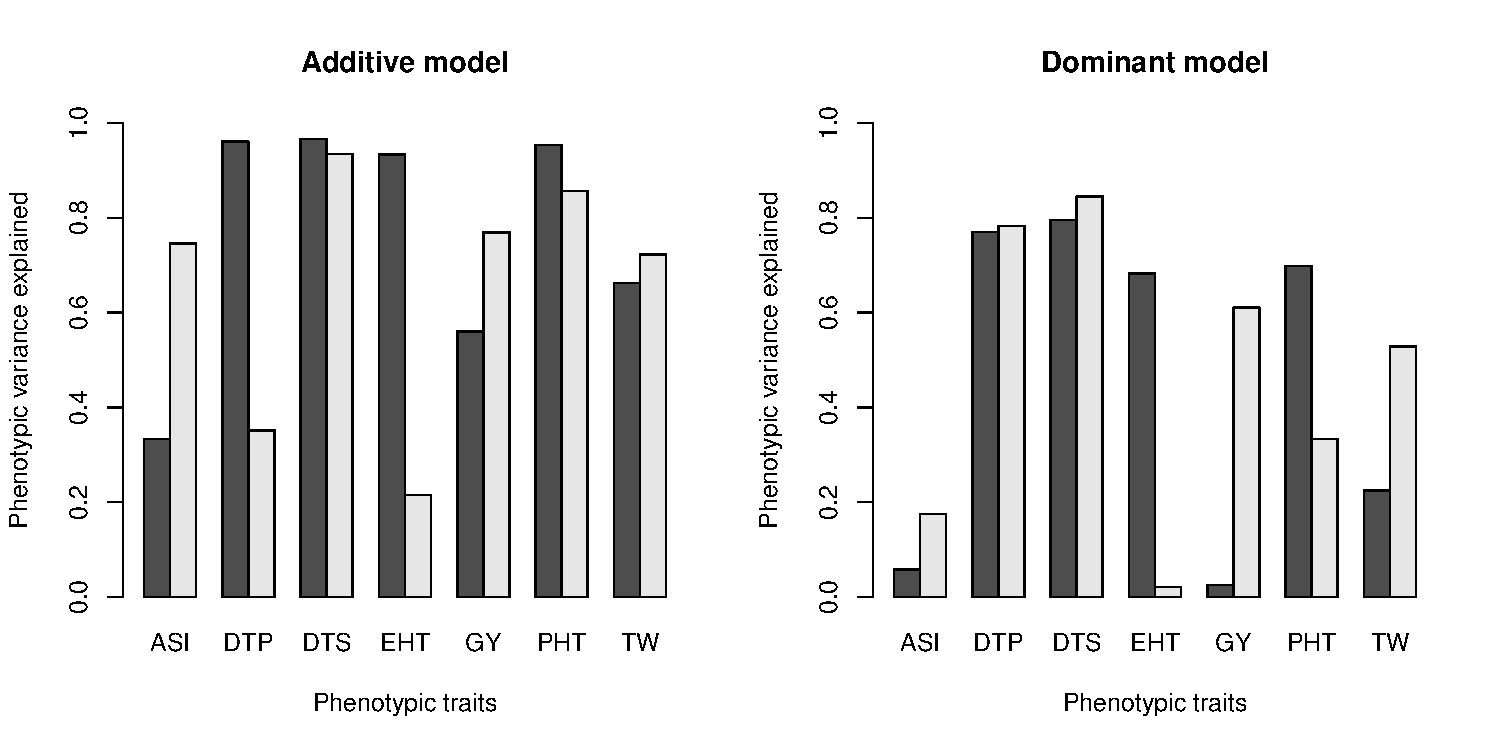
\includegraphics[width=\linewidth]{Figure_h2.pdf}
\caption{Posterior phenotypic variance explained by deleterious genic SNPs in IBD blocks using additive and dominant models. Dark color indicates trait \emph{per se} and grey color indicates BPH. }  
\label{fig:h2}
\end{figure}
%%%%%%%% ------------- %%%%%%%%%%%


%%%%%%%%%%%%%%%%%%%% DISCUSSION %%%%%%%%%%%%%%%%%%%%%%%%%%%%%%%
\section*{DISCUSSION}

In this study we have identified more than 500,000 evolutionary conserved (GERP $>$ 0) sites in the genome segregating for putatively deleterious alleles in a panel of elite maize lines. 
The non-reference alleles at these SNPs are found at low frequency, consistent with previous observations \citep{Mezmouk2014, rodgers2015recombination} and the role of selection preventing such alleles from reaching high frequency. 
Nonetheless, each inbred line carries a large number of deleterious variants, averaging $\sim 200,000$ per line. 
\jri{this should be mentioned here but also in the results. is there any big variation?  some lines more than others? is mo17 worse than the pvps? given the comment below i added about linkage, can we calculate mean deleterious variants per cM?  that would be sweet to know and to point out that there are tons around the centromere. i think a bit more detail on distribution worthwhile since even Eli's paper is only using GBS. then add here a few sentences comparing to Eli's result and McMullen 2009.}

Across lines, however, the majority of these deleterious mutations were maintained at low frequency, consistent with previous observations \citep{rodgers2015recombination}. 

The large number of linked deleterious alleles present means that there is likely insufficient recombination in standard breeding programs to completely purge all such alleles. 
Instead, breeders have devised a strategy --- hybrid breeding --- that circumvents much of this problem via complementation.
Consistent with this idea, our results show that prediction accuracies for both traits \emph{per se} as well as heterosis increased when SNPs were weighted by their likelihood of being deleterious.
Because there are likely thousands of deleterious alleles involved in complementation, many with relatively small effects, traditional GWAS approaches with genome-wide thresholds of multiple testing may not have the power to detect such effects.
Using a liberal significance threshold, however, even GWAS methods have identified an enrichment for deleterious genic SNPs among associated markers for a number of traits \citep{Mezmouk2014}.


Our models did not increase the prediction accuracies equally well for traits \emph{per se} and their heterosis transformations. 
This is not surprising, given the variation in genetic architecture of different phenotypic traits --- flowering time, for example, appears primarily determined by many loci of small additive effect \citep{buckler2009genetic}, and prediction accuracy is highest and the vast majority of phenotypic variance can be explained under simple additive models.  \jri{add other example from our data and maize lit. add sentence or two of correlation between prediction accuracies and BPH seen in boxplots -- traits with higher BPH have lower heritability and thus harder to predict normally. also add back text on how difference in prediction accuracies can be explained by heritability. why use broad sense? }

% Paritcally, with dominant model, up to 20\% of the phenotypic variance could be explained for the heterosis traits. Theoritically, BPH transformation subtracts the joint effects of the additive and dominant alleles in the best parents as residule, the substantial variance of these redidules explained by the additive or dominant models in our studies indicated that genetic components controlling for heterosis might in linked state.  

% How to explain the prediction difference?  
% The variation of the prediction accuacies were relative large in this study. First of all, broad sense heritability of the traits are different. Second, from the simulation we learned that different traits may controlled by different proportion of additive, dominant and even recessive gene actions. Our naive model only built the pure additive and pure dominant effects in. For the more complicated cases, the models may not work very well.
\jri{Here a paragraph about how additive often beat recessive and that this is consistent with a role for partial dominance. we cite Birchler arguing how complete dominance is unlikely and doesn't jive with much data. we cite Huang showing partial dominance for phenotypes per se among hybrids. can cite \citep{halligan2009spontaneous} reviewing several studies finding evidence of partial dominance. while we don't have enough power to estimate dominance, the fact that an additive model works well suggests high-ish values of h. this would be consistent with, for example, alleles affecting plant height  being predominantly additive (cite \citep{peiffer2014genetic}), but plant height is correlated with yield, so alleles affecting height will have a weak, but additive, effect on yield.  }

\jri{Discuss limitations of size of population, missing GERP data b/c of alignment with Tripsacum, missing information on non-SNP variants, etc.}
%limitation of our current models is that we assume phenotypic traits are determined by complete additive or complete dominant effects. 
%Traits with a mixture of additive and dominant casual loci may thus fail to be predicted. 
%Another limitation is likely the population size used; we may simply not have enough power to predict traits with low heritability. 
%where the haplotype was coded with the SNP conservation score as the explainatory variables. 
%Genomic variants occurred at the evolutionary constraint sites were potentially deleterious. The phenotypic effects of these genetic loads and their contributions to heterosis become an interesting area to explore. However, the population size in this study is relative small and SNPs detected at sites containing high GERP scores are generally in low frequencies. The statistical power to detect the separate effects of these putative deleterious alleles becomes very low.

As genotyping costs continue to decline, genomic prediction models are increasing in popularity \citep{desta2014genomic}. 
Most previous work on genomic prediction, however, focuses exclusively on statistical properties of the models, ignoring potentially useful biological information (but see \citex for a recent example). 
In addition to providing evidence in favor of the simple complementation model for heterosis, our work here shows the utility of incorporating functional information about the variants used in genomic prediction models.  
As our functional annotations of genomes improve, we predict that including such information in genomic prediction will be vital to the development of more powerful predictive models for plant breeding.

\section*{METHODS}
Methods and any associated references are available in a separate pdf file.

\section*{ACKNOWLEDGMENTS}
Financial support for this work came from NSF (grants IOS-0820619 and IOS-1238014), USDA (grants 2009-65300-05668 and \X), DuPont Pioneer, and N2 Genetics. We'd like to thank Graham Coop, James Holland, \X, and \X reviewers for helpful discussion.

\section*{AUTHOR CONTRIBUTIONS}
J.Y. and J.R.-I. designed this work. J.Y., T.K. and R.P.S analyzed data and T.K performed simulations. S.T., J.Y. and J.R.-I. wrote the paper.

\section*{COMPETING INTERESTS STATEMENT}
The authors declare no competing financial interests.

{\scriptsize \sf
\renewcommand{\baselinestretch}{2.0}
\bibliography{Diallel}
\bibliographystyle{NatureSeriesT}
}

\end{document}

